\section{Period Finding(Shor's Algorithm)}
\subsection{Problem}
As the name suggests, given a function $f: \{0,1\}^L \rightarrow \{0,1\}$ which is periodic with period $r$, we have to find the value of the period $r$. \\
The algorithm to solve this is known as the Shor's Algorithm. The famous application of quantum computing to break the RSA cryptosystem is based on this algorithm.
\subsection{Classical Solution}
The classical solution includes searching for the period linearly through all the values of $r$ possible. There will be $2^L$ values to be checked where $L$ is the size of input. Also, each pass would require $O(2^L)$ steps to verify whether it is the period or not. So, in total it is a $O(2^L)$ algorithm which is very-inefficient for even L in the range of thousands.
\subsection{Quantum Solution}
As we have seen till now, the use of quantum computer allows an exponential speed up. For the quantum case, we need an oracle which would perform the following operation:
\begin{equation}
U|x\rangle |y\rangle \rightarrow |x\rangle |y \oplus  f(x)\rangle
\end{equation}
\begin{figure}[h]
\centering
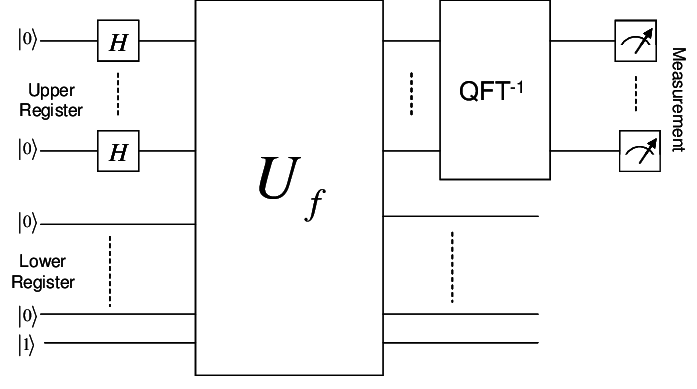
\includegraphics[width=1\textwidth]{images/shor.png}
\label{shor}
\caption{Circuit for finding the period of a given function}
\end{figure}

\\The algorithm is similar to the previous ones. We first transform the input to get the period in the phase and then use inverse QFT. The input consists of two registers similar to the phase estimation one. The first one is of sze t and is used to store the period while the second one is used to store $f(x)$ and is of size $1$.
\begin{enumerate}
\item The input is taken to be $|0\rangle |0\rangle$. 
\item Hadamard gate is used on the first register to get a superposition of all the states. So, the state becomes $$ \frac{1}{\sqrt{2^t}} \sum_{x=0}^{2^t -1} |x\rangle |0 \rangle$$
\item Then we apply the oracle to get the value of $f(x)$ in the second register. $$ \frac{1}{\sqrt{2^t}} \sum_{x=0}^{2^t -1} |x\rangle |f(x) \rangle$$ Note that the values of $f(x)$ will have a Fourier Transform say $\hat{f}(l)$ given by \begin{equation}
|\hat{f}(l)\rangle \equiv \frac{1}{\sqrt{r}} \sum_{x=0}^{r-1} e^{-2\pi ilx/r} |f(x)\rangle
\end{equation}and so \begin{equation}
|f(x)\rangle = \frac{1}{\sqrt{r}} \sum_{l=0}^{r-1} e^{2\pi ilx/r} |f(x)\rangle
\end{equation}Substituting this above we get the state as $$\frac{1}{\sqrt{r2^t}} \sum_{l=0}^{r -1} \sum_{x=0}^{2^t -1} e^{2\pi ilx/r} |x\rangle |\hat{f}(l) \rangle$$
\item If we combine the phase factor with the first register, we see that it is the inverse Fourier transform of ${l/r} $. So, we apply $QFT^{\dagger}$ to get $|\widetilde{l/r}\rangle$.
\item Measure the first register to get the value of $\widetilde{l/r}$.
\item Apply continued fraction algorithm to get the value of r.
\end{enumerate}
So, we get the value of r. The algorithm requires $O(L)$ gates to calculate the period. Next we use it to calculate the factors of a number.
\newpage
